\documentclass[onecolumn, 11pt]{article}
\setlength{\textheight}{9truein}
\setlength{\topmargin}{-0.9truein}
\setlength{\parindent}{0pt}
\setlength{\parskip}{10pt}
\setlength{\columnsep}{.4in}
\newcommand{\beq}{\begin{equation}}
\newcommand{\eeq}{\end{equation}}
\usepackage{graphicx}
\usepackage{subcaption}
\usepackage{url}

\title{Machine Learning Practise\\Playground Series - Season 3, Episode 9}
\author{Ben Colquhoun}
\date{7/3/23}
\begin{document}
\pagestyle{plain}
\maketitle
\section*{Outline of the Problem}
The task here is to predict the strength of concrete, given an instance of the concrete. This task was found as a Kaggle competition -"Playground Series - Season 3, Episode 9", joined 7 days into the 2 week duration. 
\section*{Exploratory Data Analysis}
\subsection*{Initial Features}
Inital investigation of the data provided the following features from the the training set, with expanded explanations with reference to a Kaggle discussion of Phong Nyugen \cite{feature_descriptions}. There are 5407 instances in the training dataset. 
\begin{itemize}
  \item id
  \begin{itemize}
    \item Id of the instance
    \item Integer
    \item Unimportant feature for comparing strength of concrete
  \end{itemize}
  \item CementComponent
  \begin{itemize}
    \item Amount of cement added to concrete 
    \item Float
    \item More cement improves strength of the concrete, though too much may cause it to be brittle. Important feature. 
  \end{itemize}
  \item BlastFurnaceSlag
  \begin{itemize}
    \item Amount of slag added to concrete 
    \item Float
    \item Slag can be used as a cement substitute in creating concrete. Important feature. 
  \end{itemize}
  \item FlyAshComponent
  \begin{itemize}
    \item Amount of fly ash added to concrete 
    \item Float
    \item Fly ash can be used as a cement substitute in creating concrete. Important feature.
  \end{itemize}
  \item WaterComponent
  \begin{itemize}
    \item Amount of water added to concrete 
    \item Float
    \item Water is the binding agent of the other components. Important feature. 
  \end{itemize}
  \item SuperplasticizerComponent
  \begin{itemize}
    \item Amount of superplasticizer added to concrete 
    \item Float
    \item Chemical additive to improve workability without changing water content. Reasonably important feature. 
  \end{itemize}
  \item CoarseAggregateComponent
  \begin{itemize}
    \item Amount of coarse aggregate added to concrete 
    \item Float
    \item Gravel/crushed stone added to cement for structure. Reasonably important feature. 
  \end{itemize}
  \item FineAggregateComponent
  \begin{itemize}
    \item Amount of fine aggregate added to concrete 
    \item Float
    \item Sand added to cement for structure. Reasonably important feature. 
  \end{itemize}
  \item AgeInDays
  \begin{itemize}
    \item Days since concrete poured 
    \item Integer
    \item Longer drying times increases the strength up to a point dependant on other factors. Important feature when combined with other factors. 
  \end{itemize}
\end{itemize}

All of the above features have maximum and minimum values that make sense for the context that they are in.

\subsection*{Missing Values and Duplicates}
Investigation into the duplicated values showed that there were no full instance duplications (with and without the ID), however discussions about duplicated data revealed that identical features could result in a wide variation of strength values \cite{duplicated_values}. This is evidenced by the following distributions of strength values in Figure \ref{fig:dup_distribution}. 

\begin{figure}[!ht]
  \centering
    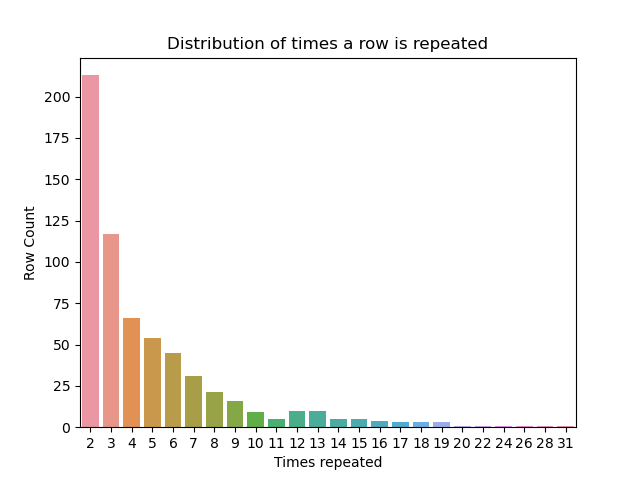
\includegraphics[width=\textwidth]{Figures/dup_number_dist.png}
  \caption{Duplicated Row Counts}
  \label{fig:dup_distribution}
\end{figure}

\begin{figure}[!ht]
  \centering
		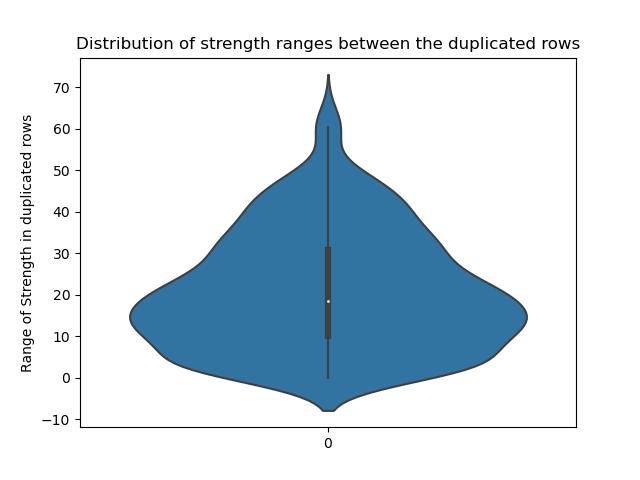
\includegraphics[width=\textwidth]{Figures/strength_range_dist.png}
  \caption{Strength Value Range over Duplicates}
	\label{fig:range_distribution}
\end{figure}

Dealing with this may require the mean strength for the duplicated row to be calculated and then input. This is especially the case as the range between the given strength values of these duplicated rows can vary wildly, as seen in Figure \ref{fig:range_distribution}.

\subsection*{Feature Engineering}
Possible feature additions have been considered and are listed below. Some of the entries are from Phong Nyugen's discussion \cite{feature_descriptions}. ChatGPT was also used to provide assistance in contextual knowledge and combinations of features. 
\begin{itemize}
  \item TotalComponentWeight = CementComponent + BlastFurnaceSlag + FlyAshComponent + WaterComponent + SuperplasticizerComponent + CoarseAggregateComponent + FineAggregateComponent
  \item Water/Cement Ratio = WaterComponent / CementComponent
  \item Aggregate Ratio = (CoarseAggregateComponent + FineAggregateComponent) / CementComponent
  \item Water/Binding Ratio = WaterComponent / (CementComponent + BlastFurnaceSlag + FlyAshComponent)
  \item Superplasticizer/Binder Ratio = SuperplasticizerComponent / (CementComponent + BlastFurnaceSlag + FlyAshComponent)
  \item Cement-Age Relation = CementComponent * AgeInDays
  \item Age Factor = Age ** n, with n some factor
 
\end{itemize}

\begin{thebibliography}{9}
  \bibitem{feature_descriptions}
  Phong Nyugen. (2023, March). \textit{Detailed feature description and feature engineering by ChatGPT}. 
  Retrieved March 7, 2023, 
  from \url{https://www.kaggle.com/competitions/playground-series-s3e9/discussion/391066}

  \bibitem{duplicated_values}
  Matt OP. (2023, March). \textit{The great duplicate saga}. 
  Retrieved March 7, 2023, 
  from \url{https://www.kaggle.com/competitions/playground-series-s3e9/discussion/391011}

\end{thebibliography}

\end{document}